\documentclass{article}
% if you need to pass options to natbib, use, e.g.:
%     \PassOptionsToPackage{numbers, compress}{natbib}
% before loading neurips_2023
\usepackage[final]{neurips}
% to avoid loading the natbib package, add option nonatbib:
%    \usepackage[nonatbib]{neurips}


\usepackage[utf8]{inputenc} % allow utf-8 input
\usepackage[T1]{fontenc}    % use 8-bit T1 fonts
\usepackage{hyperref}       % hyperlinks
\usepackage{url}            % simple URL typesetting
\usepackage{booktabs}       % professional-quality tables
\usepackage{amsmath}        % math environments and \text
\usepackage{amsfonts}       % blackboard math symbols
\usepackage{nicefrac}       % compact symbols for 1/2, etc.
\usepackage{microtype}      % microtypography
\usepackage{xcolor}         % colors
\usepackage{graphicx}       % figures
\usepackage{float}          % [H] float placement
\usepackage{tikz}           % architecture diagrams
\usetikzlibrary{positioning, calc, arrows.meta}


\title{Target-Speaker Speech-to-Text in Overlapping Speech}


\author{%
  Jibran Iqbal Shah\\
  Department of Electrical and Computer Engineering\\
  University of Toronto\\
  \texttt{jibraniqbal.shah@mail.utoronto.ca} \\
  \And
  Yamoah Frimpong Attafuah\\
  Department of Electrical and Computer Engineering\\
  University of Toronto\\
  \texttt{yamoah.attafuah@mail.utoronto.ca} \\
}

\begin{document}


\maketitle


\begin{abstract}
Modern speech-to-text systems achieve low word error rates on clean, single-speaker audio but degrade sharply when speakers overlap. We present a target-speaker speech-to-text system that, given a short enrollment clip of the desired speaker and a multi-speaker audio mixture, transcribes only the target speaker. Our pipeline combines a frozen pretrained speaker verification model (ECAPA-TDNN) to extract a speaker embedding, a trained speaker-conditioned masking network that isolates the target speaker's spectrogram, and a frozen pretrained ASR model (Whisper) for transcription. We evaluate on synthetic two-speaker mixtures from LibriSpeech at varying signal-to-interferer ratios and overlap ratios, measuring word error rate and character error rate. We show that overlapping speech degrades ASR performance across languages, and present our extraction-based approach to mitigate this degradation.
\end{abstract}

\section*{Attestation of Teamwork}
Jibran Iqbal Shah: Designed and trained the speaker-conditioned extraction network, including architecture design, loss function development (power-law compression, hybrid oracle mask loss), hyperparameter tuning, and all related code and writeup.

Yamoah Frimpong Attafuah: Fine-tuned Whisper-small on the WAXAL Akan dataset for Twi speech recognition, set up the WER evaluation scripts and notebooks, and benchmarked both the baseline Whisper and fine-tuned Whisper models across varying overlap ratios and SIR levels for English and Twi. Wrote the code and writeup related to these contributions.


\section{Introduction}

Modern speech-to-text systems perform well on clean, single-speaker audio but degrade sharply when speakers overlap~\citep{Chime, overlap}. This is a common occurrence in meetings, court proceedings, and media such as films or talk shows. Rather than attempting full diarization and separation, target-speaker transcription offers a more focused alternative: given a short enrollment clip, transcribe only the speaker of interest.

Additionally, the rise of full-duplex speech-to-speech models is increasing the demand for labelled transcriptions of natural conversations with interruptions~\citep{Moshi, PersonaPlex}. A reliable target-speaker system could automatically generate such labels by isolating each participant and producing timed transcripts, even through overlapping speech.

The objective of this project is to develop a target-speaker speech-to-text system that takes (i)~a short enrollment utterance of the target speaker and (ii)~a multi-speaker mixture, and outputs only the target speaker's transcript. We test across English and Twi to examine whether the degradation pattern is language-agnostic.


\section{Preliminaries and Problem Formulation}

Let $\mathbf{x}_{\text{mix}} \in \mathbb{R}^T$ be a single-channel audio mixture containing overlapping speech from $N \geq 2$ speakers. We are also given a short enrollment utterance $\mathbf{x}_{\text{enroll}} \in \mathbb{R}^{T_e}$ of the target speaker $s^*$. The goal is to produce a transcript $\hat{y}$ that matches the ground-truth transcript $y^*$ of speaker $s^*$ within the mixture, as measured by word error rate $\text{WER} = (S + D + I) / N_{\text{ref}}$, where $S$, $D$, $I$ are the number of substitutions, deletions, and insertions and $N_{\text{ref}}$ is the number of words in the reference transcript. Note that WER can exceed 100\% when the model produces more insertions than there are reference words.

The Short-Time Fourier Transform (STFT) converts a waveform into a two-dimensional complex-valued matrix $\mathbf{X} \in \mathbb{C}^{F \times T}$, where each entry encodes the amplitude and phase of frequency bin $f$ during time frame $t$. The magnitude spectrogram $|\mathbf{X}| \in \mathbb{R}^{F \times T}$ retains full linear frequency resolution, which is needed to invert back to a waveform after masking via the inverse STFT (iSTFT). We use standard parameters for 16\,kHz speech: 25\,ms window (400 samples), 10\,ms hop (160 samples), FFT size $N_{\text{fft}} = 512$, giving $F = 257$ frequency bins linearly spaced from 0--8000\,Hz.


\section{Design}

Our pipeline consists of three stages, illustrated in Figure~\ref{fig:pipeline}:

\begin{enumerate}
    \item \textbf{Speaker embedding extraction.} A frozen pretrained ECAPA-TDNN~\citep{ECAPA} encodes the enrollment utterance $\mathbf{x}_{\text{enroll}}$ into a speaker embedding $\mathbf{e} \in \mathbb{R}^{192}$.

    \item \textbf{Speaker-conditioned extraction.} A trained masking network receives the mixture magnitude spectrogram $|\mathbf{X}_{\text{mix}}|$ and the speaker embedding $\mathbf{e}$, and predicts a soft mask $\mathbf{M} \in [0,1]^{F \times T}$ that isolates the target speaker. The estimated target spectrogram is $|\hat{\mathbf{X}}_{\text{target}}| = \mathbf{M} \odot |\mathbf{X}_{\text{mix}}|$, and the waveform is reconstructed via iSTFT using the original mixture phase.

    \item \textbf{ASR decoding.} A frozen pretrained Whisper model transcribes the extracted waveform.
\end{enumerate}

Only the extraction network (stage 2) is trained; the speaker encoder and ASR model remain frozen throughout.

\begin{figure}[H]
\centering
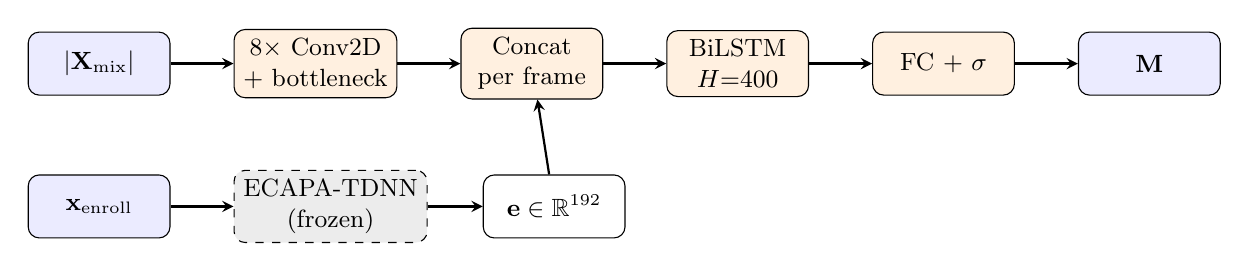
\begin{tikzpicture}[
    node distance=0.6cm and 0.9cm,
    box/.style={draw, rounded corners, minimum height=0.8cm, minimum width=1.8cm, align=center, font=\small},
    io/.style={box, fill=blue!8},
    op/.style={box, fill=orange!12},
    frozen/.style={box, fill=gray!15, dashed},
    arr/.style={-stealth, thick},
]

% Inputs
\node[io] (mag) {$|\mathbf{X}_{\text{mix}}|$};
\node[io, below=1.0cm of mag] (enroll) {$\mathbf{x}_{\text{enroll}}$};

% Speaker encoder
\node[frozen, right=0.8cm of enroll] (ecapa) {ECAPA-TDNN\\(frozen)};
\draw[arr] (enroll) -- (ecapa);

\node[box, right=0.7cm of ecapa] (emb) {$\mathbf{e} \in \mathbb{R}^{192}$};
\draw[arr] (ecapa) -- (emb);

% CNN
\node[op, right=0.8cm of mag] (cnn) {8$\times$ Conv2D\\+ bottleneck};
\draw[arr] (mag) -- (cnn);

% Concat
\node[op, right=0.8cm of cnn] (concat) {Concat\\per frame};
\draw[arr] (cnn) -- (concat);
\draw[arr] (emb) -- (concat);

% BiLSTM
\node[op, right=0.8cm of concat] (bilstm) {BiLSTM\\$H{=}400$};
\draw[arr] (concat) -- (bilstm);

% FC + sigmoid
\node[op, right=0.8cm of bilstm] (fc) {FC + $\sigma$};
\draw[arr] (bilstm) -- (fc);

% Mask output
\node[io, right=0.8cm of fc] (mask) {$\mathbf{M}$};
\draw[arr] (fc) -- (mask);

\end{tikzpicture}
\caption{Extraction network architecture. The magnitude spectrogram is encoded by eight 2D convolutional layers (with a channel bottleneck), conditioned on the speaker embedding via concatenation, and processed by a BiLSTM to predict a soft mask $\mathbf{M} \in [0,1]^{F \times T}$. Dashed box denotes a frozen pretrained model.}
\label{fig:pipeline}
\end{figure}


\section{Methodology}

\subsection{Speaker embedding}

We use a pretrained ECAPA-TDNN~\citep{ECAPA} (\texttt{speechbrain/spkrec-ecapa-voxceleb}) to extract a 192-dimensional speaker embedding from the enrollment utterance. The model achieves 0.80\% equal error rate on VoxCeleb1 and is kept frozen throughout.

\subsection{Extraction network architecture}

The extraction network follows the VoiceFilter design~\citep{VoiceFilter} and has 9.3M trainable parameters.

\subsubsection{Convolutional encoder}
The magnitude spectrogram is treated as a single-channel 2D image and processed by eight Conv2D layers, each followed by layer normalization (implemented as GroupNorm with one group) and ReLU:

\begin{table}[H]
\centering
\small
\begin{tabular}{@{}clccl@{}}
\toprule
\textbf{Layer} & \textbf{Kernel} (freq $\times$ time) & \textbf{Dilation} (freq, time) & \textbf{Ch.} & \textbf{Purpose} \\
\midrule
1 & $(7, 1)$ & $(1, 1)$ & 64 & Frequency-only \\
2 & $(1, 7)$ & $(1, 1)$ & 64 & Time-only \\
3--7 & $(5, 5)$ & $(1, 2^{k})$ & 64 & Joint, time-dilated ($k{=}0{\ldots}4$) \\
8 & $(1, 1)$ & $(1, 1)$ & 8  & Channel bottleneck \\
\bottomrule
\end{tabular}
\end{table}

Layers 1--2 are separable-style convolutions: the $(7, 1)$ kernel scans frequency to detect spectral patterns, while the $(1, 7)$ kernel scans time. Layers 3--7 use joint kernels with dilation increasing only along time (factors $1, 2, 4, 8, 16$), giving a temporal receptive field of 31 frames ($\approx$310\,ms). Layer 8 compresses from 64 to 8 channels.

Unlike 1D convolutions that treat all $F$ bins as independent channels, 2D convolutions share weights across frequency, providing frequency translation equivariance: a harmonic pattern at 500\,Hz is recognized by the same filter at 1000\,Hz.

\subsubsection{Speaker conditioning and BiLSTM}
The CNN output $\mathbf{H} \in \mathbb{R}^{B \times 8 \times F \times T}$ is flattened to $\mathbf{g}_t \in \mathbb{R}^{2056}$ per time frame. The speaker embedding $\mathbf{e} \in \mathbb{R}^{192}$ is concatenated at every frame, yielding $\tilde{\mathbf{H}}_t \in \mathbb{R}^{2248}$. A single-layer BiLSTM ($H{=}400$ per direction) processes the sequence, and two FC layers with ReLU and sigmoid produce the mask:
\begin{align}
    \mathbf{z}_t &= \text{ReLU}(\mathbf{W}_1 \mathbf{h}_t + \mathbf{b}_1) \in \mathbb{R}^{600}, \qquad
    \mathbf{M}_t = \sigma(\mathbf{W}_2 \mathbf{z}_t + \mathbf{b}_2) \in [0,1]^{F}
\end{align}

The BiLSTM is critical because overlap regions are locally ambiguous---a frame where two speakers' harmonics coincide may only be resolvable given surrounding context in both directions.

\subsection{Training objective}

\subsubsection{Power-law compressed loss}
Raw MSE loss is dominated by loud frequency bins (vowels at magnitude $\sim$10{,}000) while quiet bins (fricatives at magnitude $\sim$1) contribute negligible gradient. Following Wilson et al.~\citep{Wilson2018}, we apply power-law compression ($p = 0.3$) before computing MSE:
\[
    \mathcal{L}_{\text{recon}} = \frac{1}{FT} \bigl\| \bigl(\mathbf{M} \odot |\mathbf{X}_{\text{mix}}| + \epsilon\bigr)^{p} - \bigl(|\mathbf{X}_{\text{target}}| + \epsilon\bigr)^{p} \bigr\|_F^2
\]
where $\epsilon = 10^{-8}$ prevents gradient explosion at zero. The same compression is applied to the CNN input to normalize its dynamic range; the mask is still applied to raw magnitudes for reconstruction.

\subsubsection{Hybrid loss with oracle mask supervision}

The oracle mask is the mask that perfectly recovers the target:
$\mathbf{M}^{*}_{f,t} = \text{clamp}\!\left(|\mathbf{X}_{\text{target}}|_{f,t}\, /\, (|\mathbf{X}_{\text{mix}}|_{f,t} + \epsilon),\; 0,\; 1\right)$.
We found that power-law loss alone allows the model to find a shortcut---masks biased toward 1.0 that reduce reconstruction error without separating speakers. Adding oracle mask supervision prevents this:
\[
    \mathcal{L} = \alpha \cdot \underbrace{\|\mathbf{M} - \mathbf{M}^{*}\|_F^2}_{\text{mask MSE}} + (1 - \alpha) \cdot \mathcal{L}_{\text{recon}}
\]
We validated $\alpha = 0.1$ as optimal through controlled overfit experiments (Table~\ref{tab:hybrid}).

\subsection{Data pipeline}

\subsubsection{Datasets}
We use two speech corpora. \textbf{LibriSpeech}~(English): read speech derived from public-domain audiobooks, 16\,kHz mono. We use the \texttt{dev-clean} and \texttt{test-clean} splits. \textbf{WAXAL Akan}~(Twi): a dataset of Twi speech from the HuggingFace Hub, used to fine-tune Whisper for a language it does not natively support. All audio is loaded at 16\,kHz and peak-normalized to $[-1, 1]$.

\subsubsection{Synthetic mixture generation}
We generate 12{,}500 two-speaker mixtures from LibriSpeech by summing pairs of utterances from different speakers:
$\mathbf{x}_{\text{mix}} = \mathbf{x}_{\text{target}} + \alpha\,\mathbf{x}_{\text{interferer}}$,
where $\alpha$ controls the signal-to-interferer ratio (SIR). We vary SIR $\in \{0, 5\}$\,dB and overlap ratio $\in \{0.1, 0.2, 0.3, 0.4, 0.5, 1.0\}$. The overlap ratio determines what fraction of the target utterance is overlapped by the interferer. Each mixture preserves the aligned clean target waveform for computing oracle masks and ground-truth spectrograms during training.

\subsubsection{Train/validation/test split}
The 12{,}500 recipes are split into 10{,}000 train, 1{,}250 validation, and 1{,}250 test samples. Speaker embeddings for all unique enrollment utterances (2{,}588 embeddings) are precomputed and cached.


\section{Numerical Experiments}

\subsection{Whisper fine-tuning for Twi}

Whisper does not natively support Twi (Akan), producing near-100\% WER and CER out of the box. We fine-tuned Whisper-small (244M params) on the WAXAL Akan dataset, reducing clean-speech WER from $\sim$100\% to 33.3\% and CER from $\sim$100\% to 12.1\%. This fine-tuned model serves as the Twi baseline for our overlap experiments.

\subsection{Baseline: overlap degrades ASR across languages}

We evaluated Whisper-tiny (39M params) on English and the fine-tuned Whisper-small on Twi across all SIR levels and overlap ratios.

\begin{figure}[H]
\centering

\includegraphics[width=0.48\textwidth]{English_Base_Whisper_WER_vs_Overlap.png}
\hfill

\includegraphics[width=0.48\textwidth]{Twi_Finetuned_Whisper_WER_vs_Overlap.png}
\caption{WER vs.\ overlap ratio for English (left) and Twi (right) at three SIR levels. Both languages show the same degradation pattern: WER increases with overlap ratio and decreases with SIR. At 0\,dB SIR with full overlap, English WER exceeds 100\%.}
\label{fig:baseline-wer}
\end{figure}

English clean baseline: 8.1\% WER. At 0\,dB SIR with full overlap, WER exceeds 100\%. Twi clean baseline: 34.7\% WER with the same degradation pattern. This confirms the problem is language-agnostic.

\subsection{Hybrid loss validation}

We validated the hybrid loss weight $\alpha$ through controlled overfit experiments (seed=42, 1 batch of 16 samples, 200 epochs, lr=$10^{-4}$, compressed input) with dual-metric logging.

\begin{table}[H]
  \caption{Hybrid loss ablation on 1-batch overfit test ($p = 0.3$, 200 epochs).}
  \label{tab:hybrid}
  \centering
  \small
  \begin{tabular}{cccl}
    \toprule
    $\alpha$ & Recon PL & Mask MSE & Notes \\
    \midrule
    0.0 (power-law only) & \textbf{0.0027} & 0.333 & Best recon, but masks diverge \\
    0.05 & 0.0031 & 0.0171 & \\
    \textbf{0.1} & 0.0032 & \textbf{0.0166} & \textbf{Best balance} \\
    0.2 & 0.0033 & 0.0155 & \\
    1.0 (oracle only) & 0.0046 & 0.0184 & Good masks, poor recon \\
    \bottomrule
  \end{tabular}
\end{table}

The key finding: power-law loss alone ($\alpha = 0$) achieves the best reconstruction metric but produces masks biased toward 1.0 (mask MSE of 0.333 vs.\ all-ones baseline of 0.158), meaning the model learns to pass everything through rather than separate speakers. Adding 10\% oracle mask supervision ($\alpha = 0.1$) reduces mask MSE by $20\times$ with only a 19\% increase in reconstruction loss.

\subsection{Training}

We trained with the validated configuration: batch size 32, learning rate $10^{-3}$ with ReduceLROnPlateau (factor 0.5, patience 3), Adam optimizer, hybrid loss $\alpha = 0.1$, power-law compression $p = 0.3$, early stopping with patience 7.

% TODO: Add training curves (train loss, val loss vs epoch)
% TODO: Add final training results

\subsection{WER evaluation with extraction}

We evaluated two trained models on the 1{,}250-sample test set: the hybrid loss model ($\alpha = 0.1$) and the power-law reconstruction loss model ($\alpha = 0$). Both were trained until validation loss plateaued.

\begin{figure}[H]
\centering
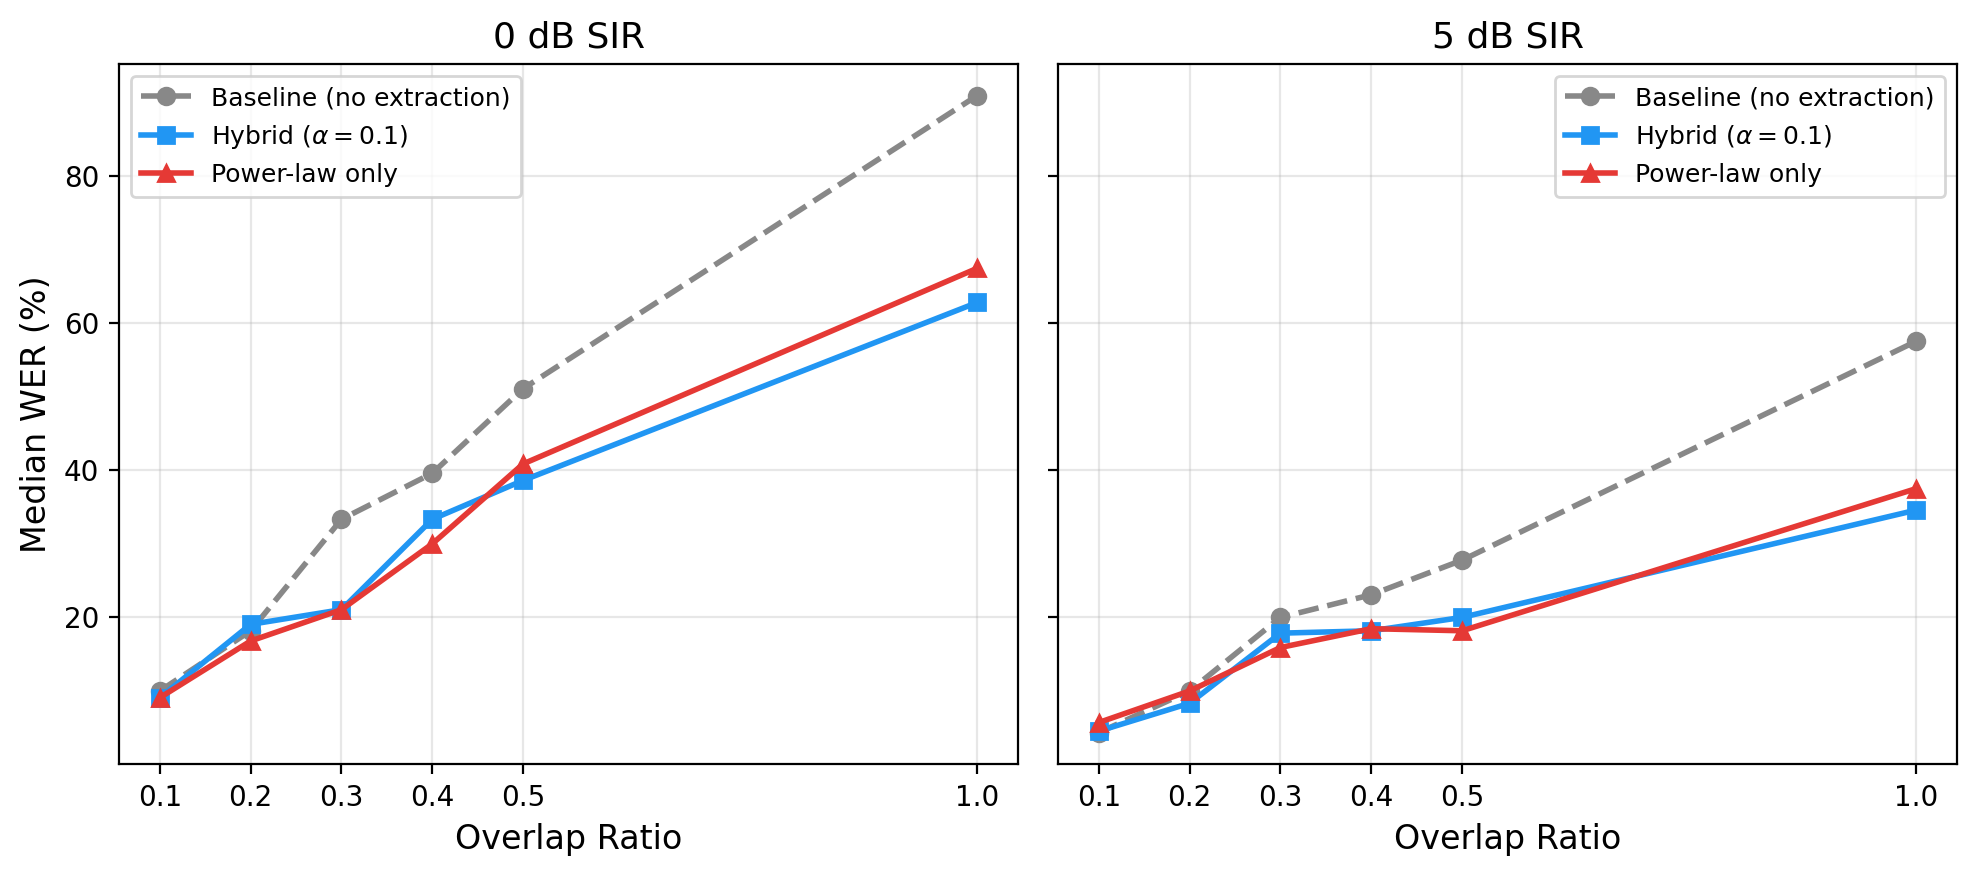
\includegraphics[width=\textwidth]{extraction_wer_comparison.png}
\caption{Median WER vs.\ overlap ratio for baseline (no extraction), hybrid loss ($\alpha = 0.1$), and power-law reconstruction loss only ($\alpha = 0$) at 0\,dB SIR (left) and 5\,dB SIR (right). Both extraction models reduce WER at overlap ratios $\geq 0.3$, with the largest gains at full overlap.}
\label{fig:extraction-wer}
\end{figure}

Both extraction models significantly reduce median WER compared to the baseline at overlap ratios $\geq 0.3$. At full overlap (1.0), the hybrid model reduces WER from 90.9\% to 62.8\% at 0\,dB and from 57.5\% to 34.6\% at 5\,dB. The power-law model achieves comparable gains (67.4\% and 37.5\% respectively). Neither model consistently dominates the other: hybrid is slightly better at very high overlap (1.0), while power-law is slightly better at medium overlap (0.3--0.5). At low overlap ($\leq 0.2$), extraction provides marginal or no benefit, as the interference is brief enough for Whisper to handle without assistance.


\section{Discussion}

The extraction network reduces WER most where baseline Whisper struggles most: at high overlap ratios and low SIR. At 0\,dB SIR with full overlap, median WER drops from 90.9\% to 62.8\%, a 28 percentage point reduction. At 5\,dB SIR with full overlap, the reduction is 57.5\% to 34.6\%. The difference between the hybrid loss ($\alpha = 0.1$) and pure power-law reconstruction loss ($\alpha = 0$) is minimal in terms of downstream WER, suggesting that the choice of training objective matters less than the overall extraction approach.

However, the extracted WER at full overlap (62.8\% at 0\,dB) remains far from the clean-speech baseline of 8.1\%. The model has not fully converged during training: the validation loss plateaued well above the oracle mask floor, indicating that the predicted masks are still far from optimal. Longer training, higher model capacity, or architectural improvements such as skip connections could close this gap.

Our training data was uniformly distributed across overlap ratios (0.1, 0.2, 0.3, 0.4, 0.5, 1.0), meaning the model spent equal time on easy cases (low overlap, where Whisper already performs well) and hard cases (high overlap, where extraction is most needed). Biasing the training distribution toward higher overlap ratios, or using a curriculum that starts with easy examples and gradually increases difficulty, could improve performance on the conditions where extraction matters most.

We demonstrated that overlapping speech degrades ASR in both English and Twi, confirming the problem is language-agnostic. The extraction network operates on spectrograms and speaker embeddings rather than language-specific features, so it should in principle generalize across languages. We did not have time to evaluate the extraction network on Twi, but this is a natural next step: training on English and testing on Twi would reveal whether the learned masking strategy transfers cross-lingually without additional fine-tuning.

\section{Conclusions}

We built a target-speaker speech-to-text system that uses a speaker-conditioned masking network to isolate a target speaker from a two-speaker mixture before transcription with Whisper. The system reduces median WER by up to 28 percentage points at full overlap compared to running Whisper directly on the mixture. We showed that speaker overlap degrades ASR performance in both English and Twi, and that a lightweight extraction module (9.3M parameters) trained with a hybrid loss can partially recover the target speaker's signal. Future work should explore curriculum learning, harder training distributions, and cross-lingual evaluation to improve performance on the most challenging conditions.


\bibliographystyle{unsrtnat}
\bibliography{references}


\newpage
\section*{Use of AI}
% TODO: Describe AI usage
We used Claude Code (Anthropic) as a coding assistant throughout the project for implementing the extraction network architecture, debugging training issues, writing evaluation scripts, and drafting sections of this report. All AI-generated code was reviewed, tested, and modified by the authors. Architecture decisions (hybrid loss formulation, 2D CNN design, hyperparameter choices) were made by the authors based on experimentation and literature review, with AI assistance for implementation.


\section*{Consent for Information Sharing}

\begin{itemize}
	\item All group members consent to allow the project materials (report, slides, and presentation recording) to be shared on the course page for future students.
\end{itemize}


\section*{Consent for Use of Project Information in Statistical Analysis}
\begin{itemize}
	\item All group members consent to allow anonymized information about the project (e.g., topic, methods, outcomes, grades) to be used by the instructor for statistical analysis and course improvement.
\end{itemize}

\subsection*{Group Identification}

\begin{itemize}
	\item Group number: 28
	\item Names of group members: Jibran Iqbal Shah, Yamoah Frimpong Attafuah
	\item Signature of group members: Jibran Iqbal Shah, Yamoah Frimpong Attafuah
	\item Date: April 10, 2026
\end{itemize}

\end{document}
